\section{Minkowski-diagrammen}

%afbeeldingen draaien enz.
% 5.6 toevoegen.

%%%%%%%%
\subsection{Drie gebeurtenissen}
Gebeurtenissen worden vanuit drie standpunten bekeken die een onderlinge 
beweging hebben: $S_{1}$, $S_{2}$ en $S_{3}$. 

% \begin{figure} [h]
% \begin{center}
% \mbox{\epsfxsize=10cm\epsffile{oefeningen.pictures/oef_4/oef4-1.eps}}
% \caption{Drie gebeurtenissen}
% \label{f:oef4-1}
% \end{center}
% \end{figure}

\begin{figure}[ht]
\centering
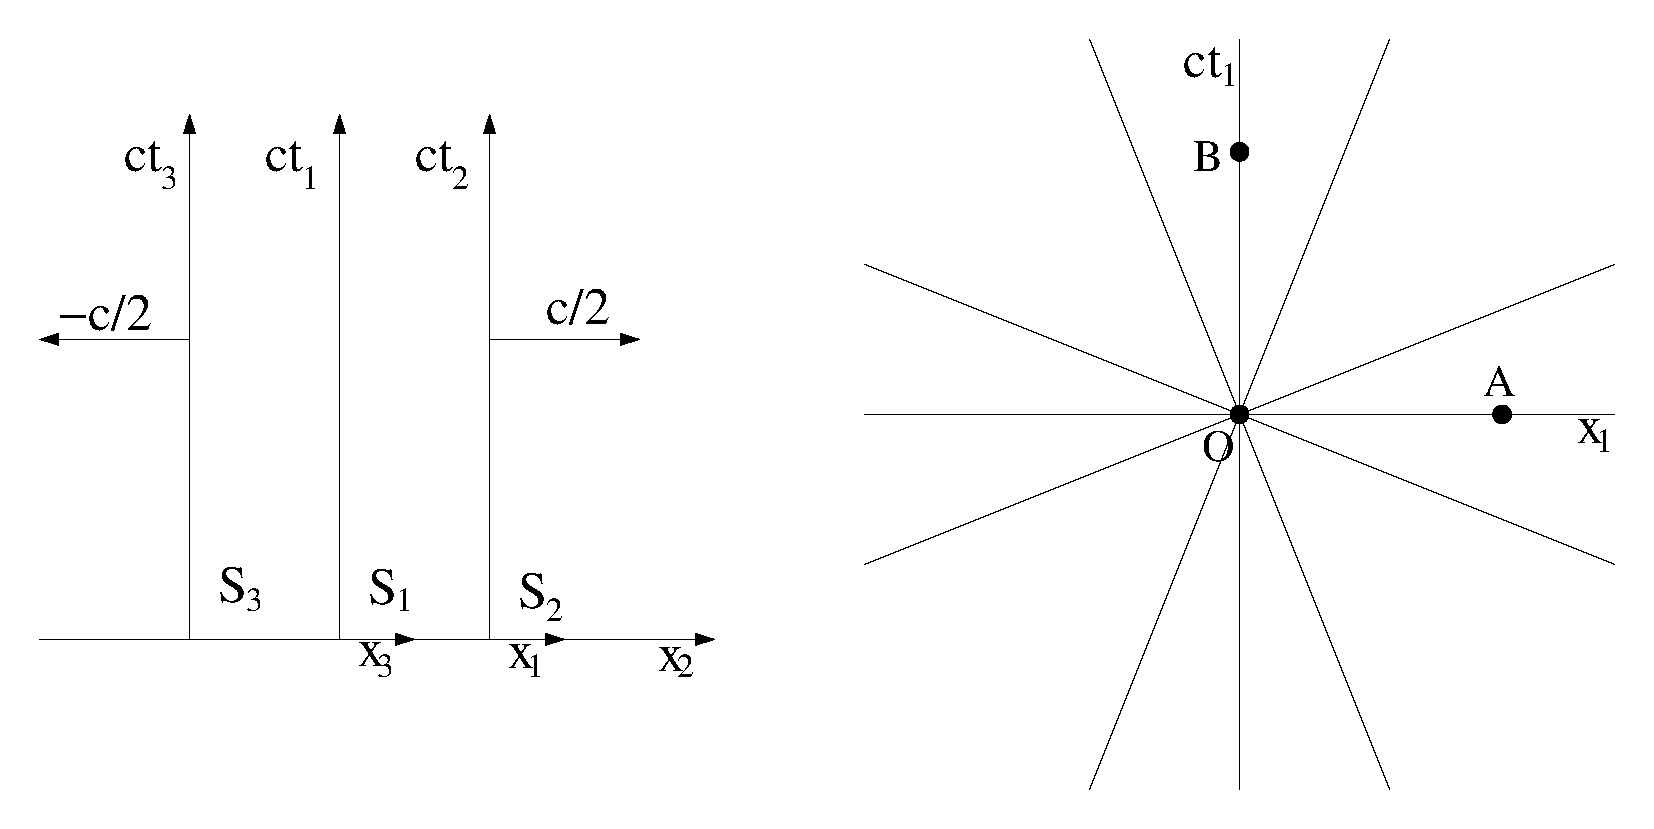
\includegraphics[width=.8\textwidth]{oefeningen.pictures/oef_4/oef4-1}
\caption{Drie gebeurtenissen}
\label{f:oef4-1}
\end{figure}  

In het Minkowski-diagram van $S_{1}$ zijn drie "gebeurtenissen" $O$, $A$ en $B$
aangegeven. 
\begin{itemize}
\item [a.]
  Geef in het rechter diagram aan wat de $x_{2}$-, $ct_{2}$-, $x_{3}$- en
  $ct_{3}$-assen zijn. 
\item  [b.]
  Volgens $S_{1}$ is gebeurtenis $A$ gelijktijdig met gebeurtenis $O$. 
Hoe zit dat in $S_{2}$ en $S_{3}$? 
\item [c.]
  In  $S_{1}$ stelt de overgang van $O$ naar $B$ een toestand van rust voor. 
Hoe zit dat in $S_{2}$ en in $S_{3}$? 
\end{itemize}

%%%%%%%
\subsection{Draaing in het $ct,x$-diagram}
We kijken naar twee stelsels $S$ en $S'$ die verbonden zijn door de 
Lorentztransformatie (zie figuur \ref{f:rotate}):
\begin{eqnarray*}
   x & = & \gamma (x' + \beta ct')  \\
  ct & = & \gamma(ct'+\beta x')
\end{eqnarray*}  

% \begin{figure} [h]
% \begin{center}
% \mbox{\epsfxsize=10cm\epsffile{oefeningen.pictures/oef_4/rotate.eps}}
% \caption{Draaiing van assen}
% \label{f:rotate}
% \end{center}
% \end{figure}

\begin{figure}[ht]
\centering
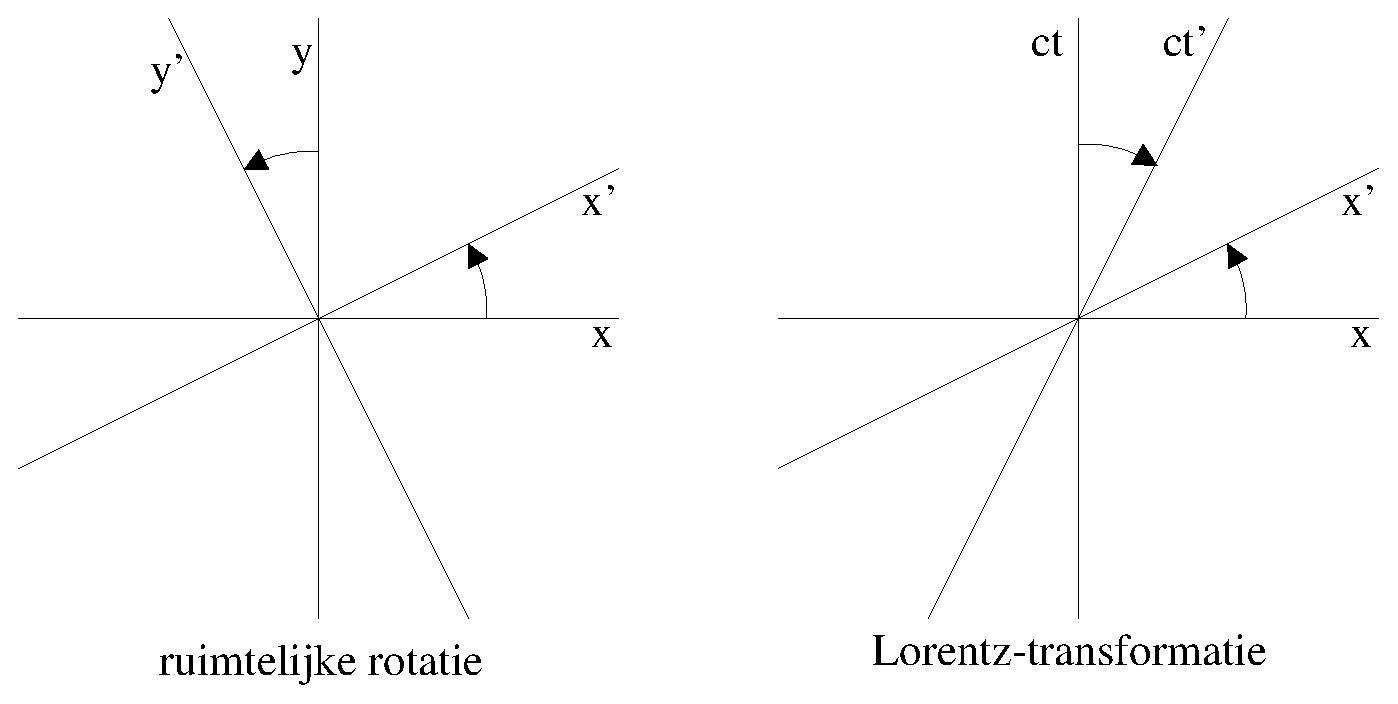
\includegraphics[width=.8\textwidth]{oefeningen.pictures/oef_4/rotate}
\caption{Draaiing van assen}
\label{f:rotate}
\end{figure}

De  Lorentztransformatie  veroorzaakt  een soort draaiing in het 
$ct$,$x$-diagram, die lijkt op een 
gewone  ruimtelijke  rotatie in het $x,y$-vlak, met het verschil dat 
de $ct$- en $x$-assen beide naar 
binnen draaien, over een hoek $\alpha$ met $\tan{\alpha} = \beta = v/c$ :

\begin{itemize}
\item [a.]
  Laat  zien  dat  de  $x'$-as  (de  lijn  met  $ct' = 0$)  in  het  
$ct$,$x$-diagram  een lijn met 
  richtingsco\"{e}ffici\"{e}nt $\beta$ is (dus van de vorm $ct = \beta x$ is).
\item [b.]
  Laat ook zien dat de $ct'$-as (dus de lijn met $x' = 0$) een
  richtingsco\"{e}ffici\"{e}nt $\beta$ heeft met de 
  $ct$-as (dus van de vorm $x = \beta ct$ is).
\end{itemize}

Terwijl  bij  een  rotatie  in  het  $x,y$-vlak  de  eenheden  op de 
gedraaide assen liggen op de eenheidscirkel  $x^{2} + y^{2} = 1$,  
zo liggen de eenheden van de gekantelde $ct'$,$x'$-assen op de eenheids 
hyperbolen $x^{2} - (ct)^{2}= \pm 1$ (figuur \ref{f:eenheid}):

% \begin{figure} [h]
% \begin{center}
% \mbox{\epsfxsize=10cm\epsffile{oefeningen.pictures/oef_4/eenheid.eps}}
% \caption{Eenheden}
% \label{f:eenheid}
% \end{center}
% \end{figure}

\begin{figure}[ht]
\centering
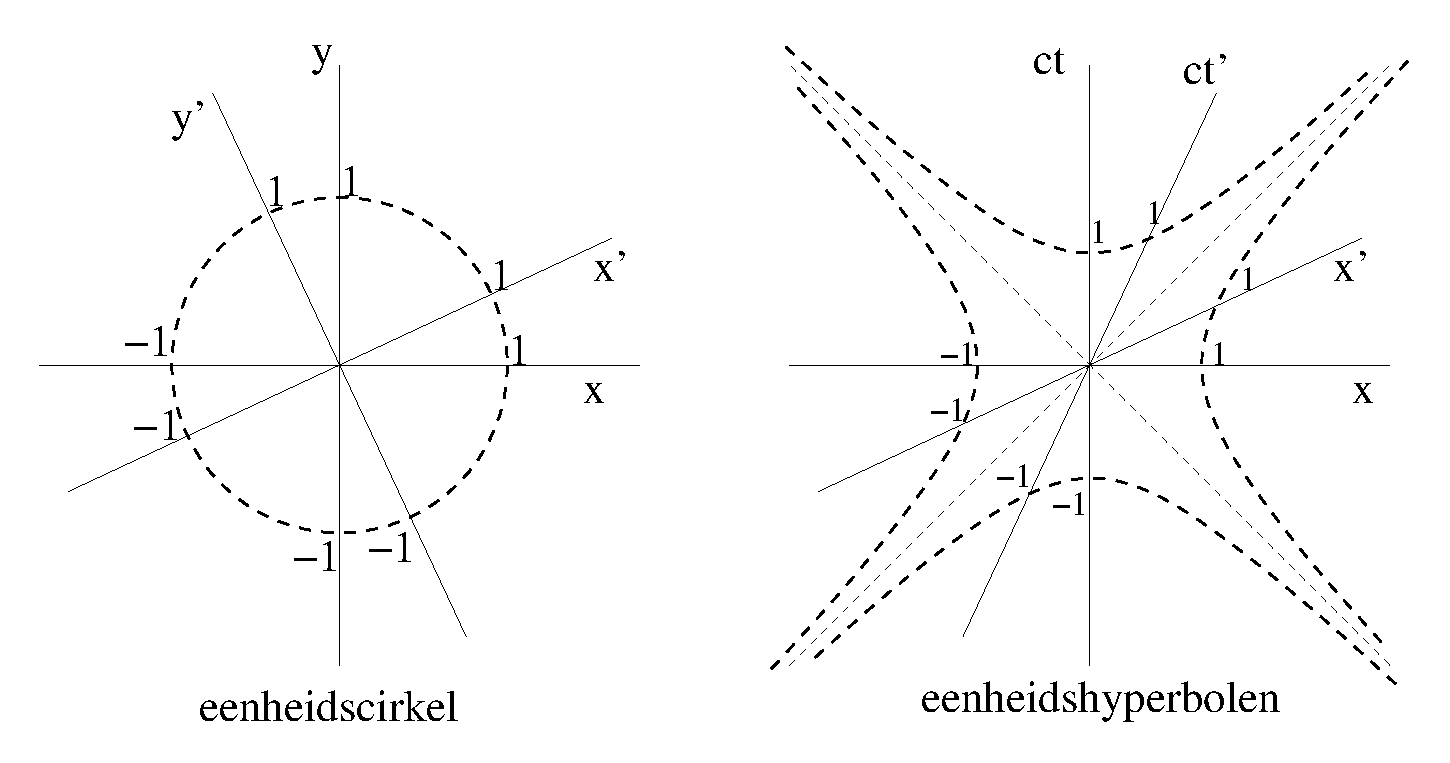
\includegraphics[width=.8\textwidth]{oefeningen.pictures/oef_4/eenheid}
\caption{Eenheden}
\label{f:eenheid}
\end{figure}

%eenheids-                                      eenheids-
% cirkel                                       hyperbolen
%$x_{1}^{2}+y_{1}^{2}=1$                    $x_{1}^{2}-(ct_{1})^{2}=\pm 1$

\begin{itemize}
\item [c.]
  Reken  voor  de  eenheden  op de $x'$-as (dus $ct' = 0$ en
  $x' = \pm 1$) na dat de bijbehorende $x$- en 
  $ct$-getallen voldoen aan $x^{2} - (ct)^{2} = +1$.
\item [d.]
  Hetzelfde voor de eenheden op de $ct'$-as: $x^{2} - (ct)^{2} = -1$.
\end{itemize}


%%%%%%%%%%
\subsection{Lorentzcontractie en Tijddilatatie in Minkowski-diagram}


%\begin{figure}[ht]
%\centering
%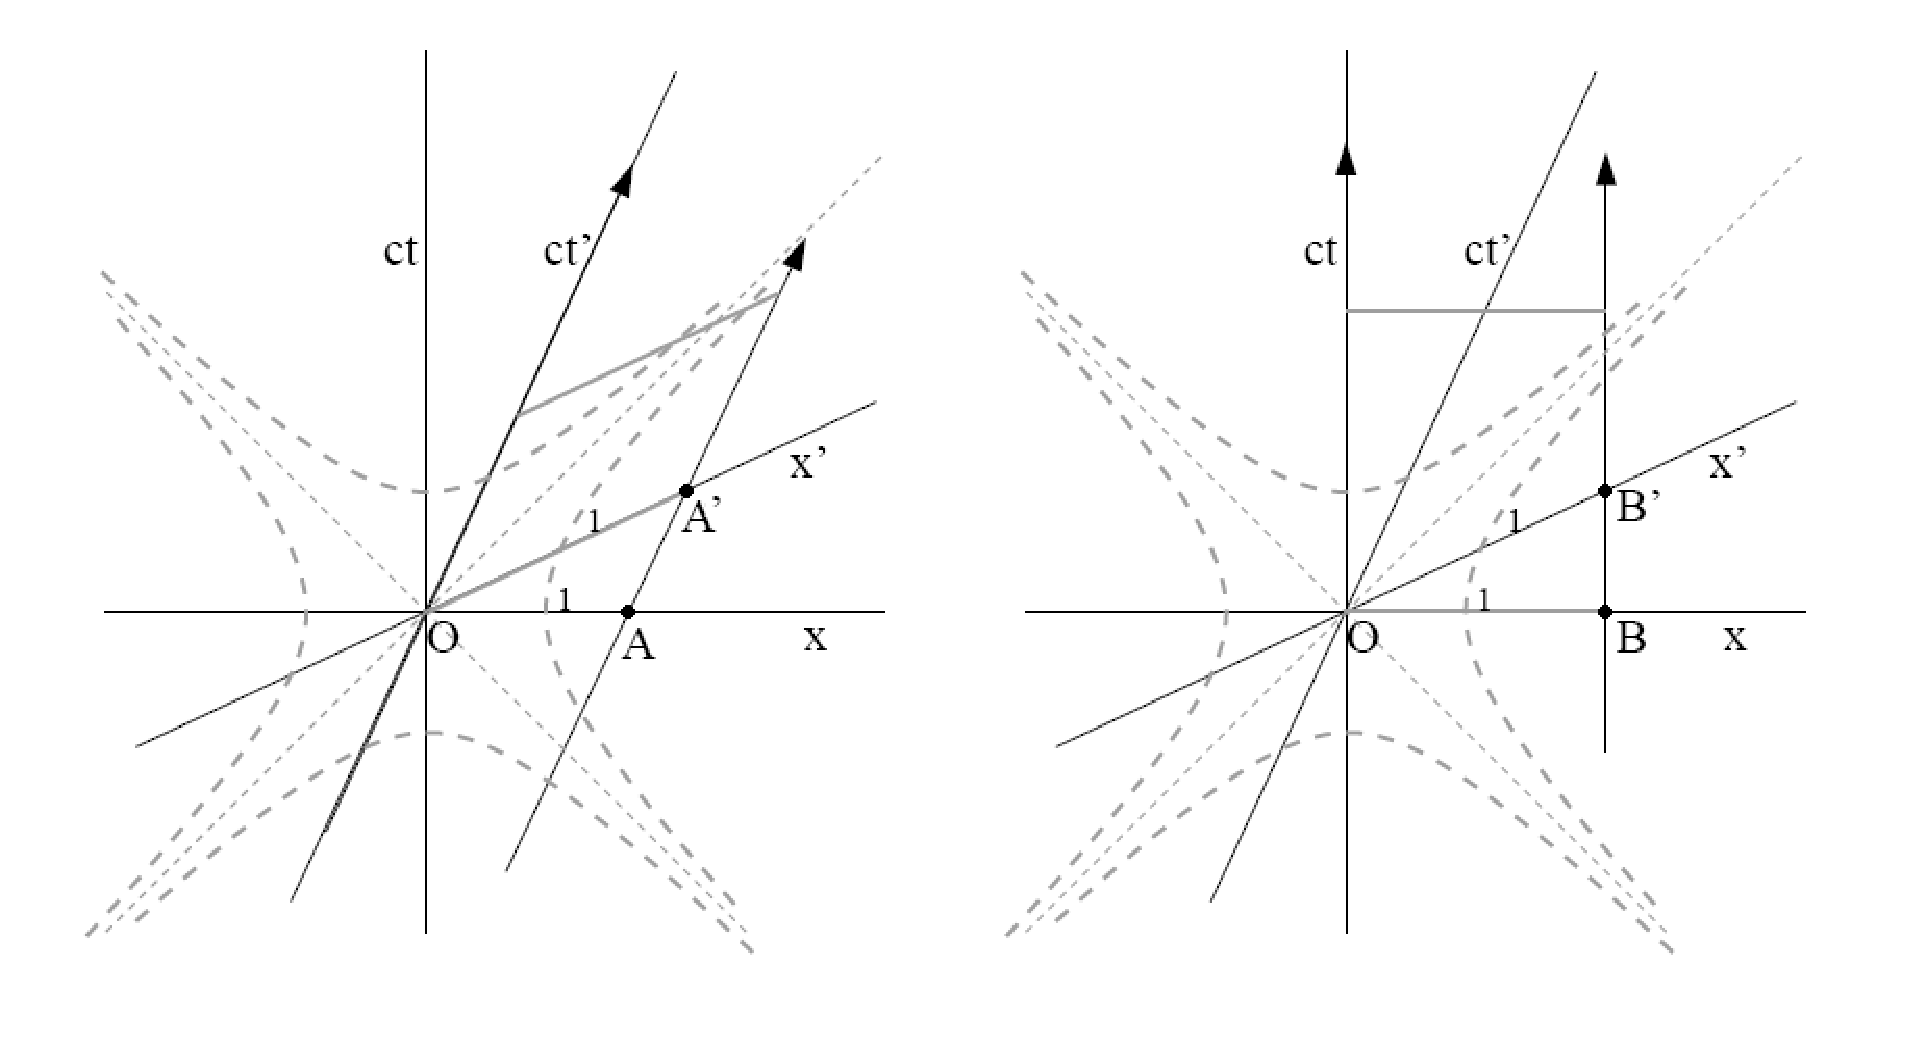
\includegraphics[width=0.8\textwidth]{contractiediag1}
%\caption{Lorentzcontractie}
%\label{f:mcontractie}
%\end{figure}

\begin{figure}[ht]
 \begin{center}
 \mbox{\epsfxsize=10cm\epsffile{oefeningen.pictures/contractiediag1.eps}}
 \caption{Tijddilatatie}
 \label{f:mcontractie}
 \end{center}
 \end{figure}


 Lorentzcontractie met een Minkowski-diagram: 
\begin{itemize}
\item [a.]
 Toon  met  de  twee diagrammen van figuur \ref{f:mcontractie} aan dat een 
lat $OA'$
 (met lengte 2) in $S'$, gezien vanuit $S$ verkort 
 is, en andersom, dat een lat $OB$ in $S$, verkort is in $S'$.
\end{itemize}

%\begin{figure}[h]
%	\centering
%		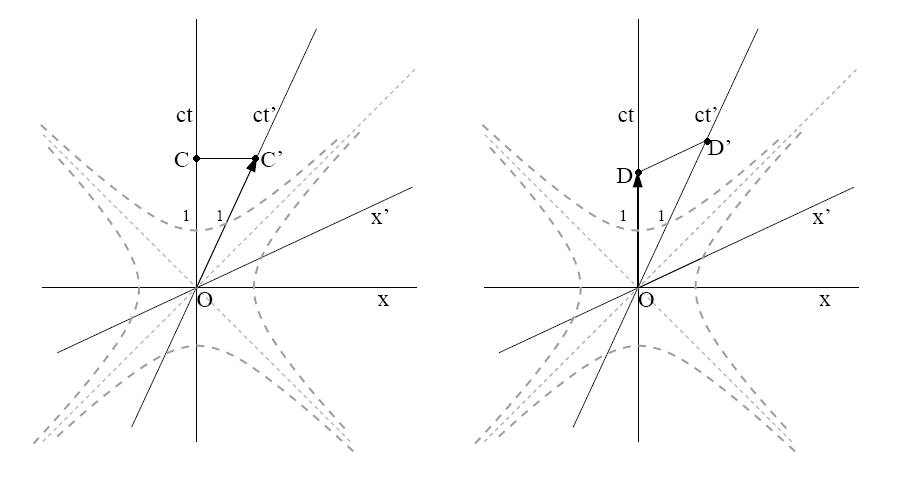
\includegraphics[width=0.8\textwidth]{contractiediag2.EPS}
%	\caption{Tijddilatatie}
%	\label{f:mtijddil}
%\end{figure}

 \begin{figure}[ht]
 \begin{center}
 \mbox{\epsfxsize=10cm\epsffile{oefeningen.pictures/contractiediag2.eps}}
 \caption{Tijddilatatie}
 \label{f:mtijddil}
 \end{center}
 \end{figure}

  Tijddilatatie in een Minkowski-diagram:
\begin{itemize}
\item [b.]
Laat in de diagrammen van figuur \ref{f:mtijddil} zien dat een klok, 
die in $S'$ van $O$ naar $C'$ loopt, vanuit $S$ gezien langzamer is, 
en andersom, dat een klok die in $S$ van $O$ naar $D$ loopt, vanuit $S'$ gezien 
langzamer is.
\end{itemize}


%%%%%%%%%%%
\subsection{Wereldlijnen}
In  het  co\"{o}rdinatenstelsel $S$ staan $A$ en $B$ stil op de plaatsen
$x_{A} = 0$ en $x_{B} = 3$. 
Op $t = 0$ zendt $A$ 
een lichtgolf uit die $B$ bereikt op $t = \frac{3}{c}$. 

% \begin{figure} [h]
% \begin{center}
% \mbox{\epsfxsize=10cm\epsffile{oefeningen.pictures/oef_4/kleurplaat.eps}}
% \caption{Teken wereldlijnen}
% \label{f:kleurplaat}
% \end{center}
% \end{figure}


\begin{figure}[ht]
\centering
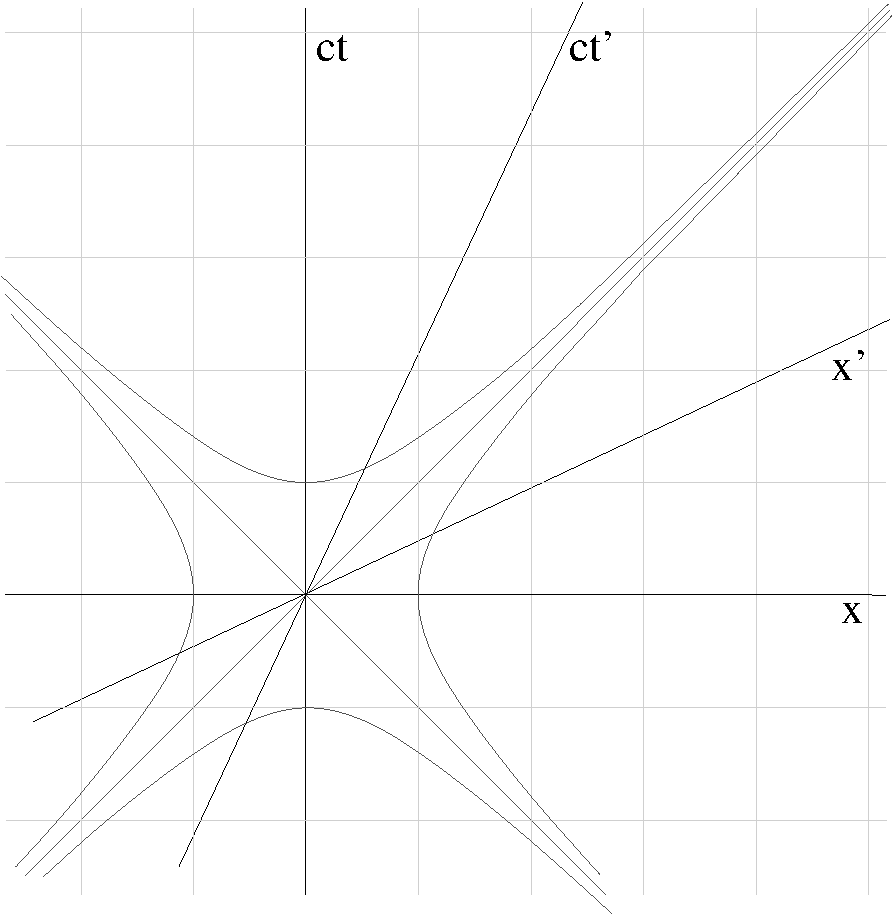
\includegraphics[width=.8\textwidth]{oefeningen.pictures/oef_4/kleurplaat}
\caption{Teken wereldlijnen}
\label{f:kleurplaat}
\end{figure}

\begin{itemize}
\item [a.]
  Teken in het Minkowski-diagram in figuur \ref{f:kleurplaat}
  de zgn. wereldlijnen van $A$ en $B$ 
(dus de lijnen $x = 0$ 
  en $x = 3$). Teken ook het punt $C$: de gebeurtenis waar het licht vanuit $A$, $B$ bereikt. 
\end{itemize}
Een  ander stelsel $S'$ beweegt met $\frac{1}{2}c$ t.o.v. $S$ in de positieve 
$x$-richting.
De $x'$,$ct'$-assen zijn 
al in het diagram aangegeven. 

\begin{itemize}
\item [b.]
  Controleer dat de snelheid van $S'$ t.o.v. $S$ gelijk is aan $\frac{1}{2}c$ 
  en geef 
het punt $B'$ aan waar 
  $B$ zich volgens $S'$ bevindt op het ogenblik dat het licht uit $A$ 
vertrekt. 
\item [c.]
  Bereken  de  $ct'$,$x'$  co\"{o}rdinaten  voor  de  punten  $B'$  en  $C$ 
(gebruik daarbij de Lorentztransformatie) 
\item [d.]
  Bereken uit de $x'$- en $t'$-verschillen tussen $B'$ en $C$ hoe snel $B$ 
beweegt in $S'$; bereken uit 
  de  $x'$-  en  $ct'$-verschillen  tussen de oorsprong $O$ en $C$ hoe groot 
de lichtsnelheid in $S'$ is. 
  Waren deze antwoorden te verwachten? 
\end{itemize}

%%%%%%%%%%%%%
\subsection{Opnieuw raketten}
Nog een keer de situatie van de opgave `Raketten 2' (opgave \ref{prob:rak4}).

% \begin{figure} [h]
% \begin{center}
% \mbox{\epsfxsize=10cm\epsffile{oefeningen.pictures/oef_4/kleurplaat.eps}}
% \caption{Teken raketbewegingen}
% \label{f:kleurplaat2}
% \end{center}
% \end{figure}

\begin{figure}[ht]
\centering
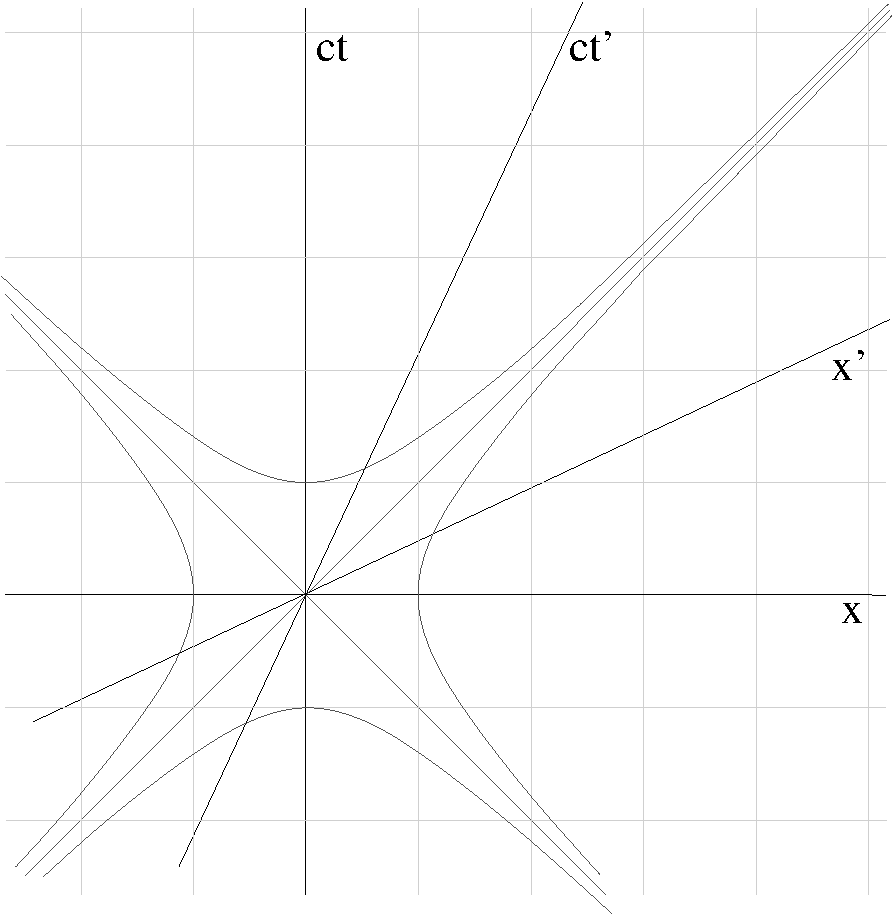
\includegraphics[width=.8\textwidth]{oefeningen.pictures/oef_4/kleurplaat}
\caption{Teken raketbewegingen}
\label{f:kleurplaat2}
\end{figure}

\begin{itemize}
\item [a.]
Teken de beweging van $P$ en $Q$ in het Minkowski-diagram in figuur \ref{f:kleurplaat2}. 
 
\item [b.]
  Teken de $x'$,$ct'$ assen die gelden voor een waarnemer ($S'$) die met 
raket $P$ mee beweegt. 
\item [c.]
  Hoe groot is volgens $S'$ op $t' = 0$ de afstand $x'$ tot raket $Q$? 
(uit het diagram aflezen) 
\item [d.]
  Na hoeveel tijd ontmoeten $P$ en $Q$ elkaar in $S'$? (uit het diagram
  aflezen).
\item [e.]
Bereken  de  snelheid  van  $Q$  in  $S'$  uit  de $x'$-verplaatsing van $Q$
tussen $ct' = 0$ en zijn ontmoeting met $P$. 
Vergelijk het antwoord met vraag d) van de opgave `Raketten' uit hoofdstuk \ref{CLT}.
\end{itemize}

%\newpage
%Gebruik voor het huiswerk onderstaande figuur.
%
%% \begin{figure} [h]
%% \begin{center}
%% \mbox{\epsfxsize=10cm\epsffile{oefeningen.pictures/oef_4/kleurplaat.eps}}
%% \caption{Teken raketbewegingen}
%% \end{center}
%% \end{figure}
%
%\begin{figure}[ht]
%\centering
%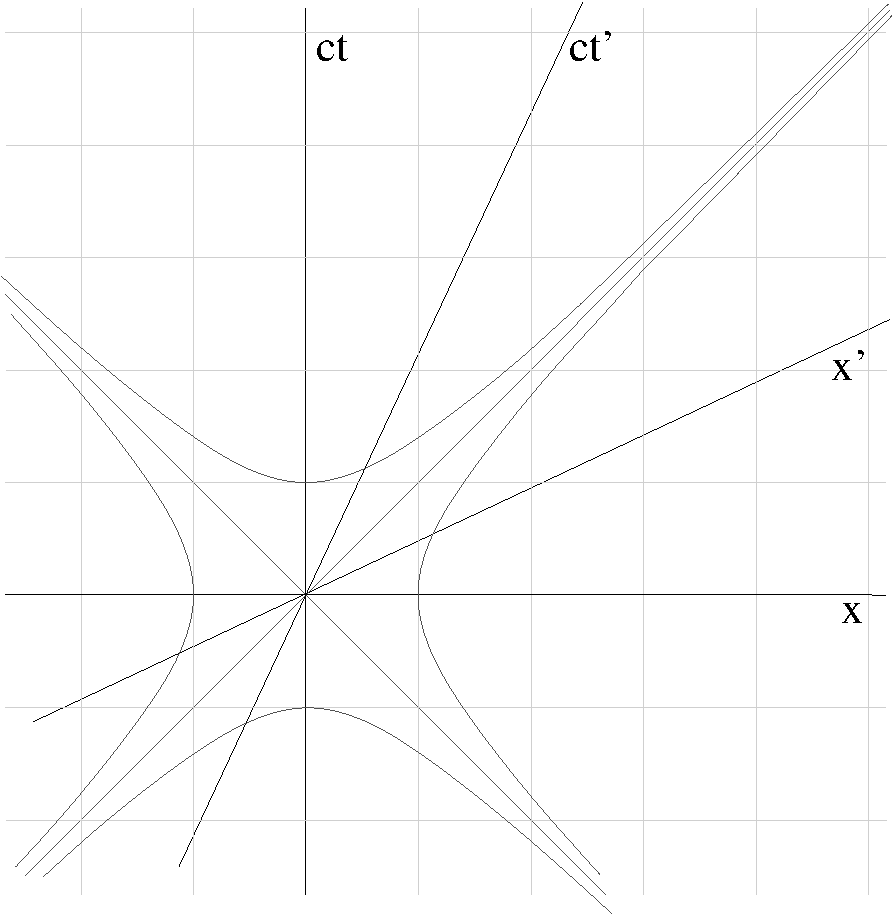
\includegraphics[width=1.0\textwidth]{oefeningen.pictures/oef_4/kleurplaat}
%\caption{Teken raketbewegingen}
%\end{figure}

%%%%%%%%%
\subsection{Nogmaals raketten}

			Hieronder zie je twee onvolledige Minkowski-diagrammen, die horen bij de eerder gemaakte opdracht \ref{prob:rak3}. Het ene diagram
toont de situatie zoals waargenomen vanuit $S$, de andere zoals waargenomen
vanuit $S'$. Geef in beide diagrammen aan of de assen $ct'$ of $x'$, danwel $ct$ of $x$ zijn. Geef verder in
ieder van de diagrammen aan wat de wereldlijnen zijn van $P$ en $Q$. Teken ten
 slotte in ieder van de diagrammen een lichtstraal die uitgezonden wordt
door $P$ in de richting van $Q$ (de aankomst van de lichtstraal bij $Q$ zou
buiten de tekening kunnen vallen).
			
			

 \begin{figure} [h]
 \begin{center}
 \mbox{\epsfxsize=14cm\epsffile{oefeningen.pictures/MinkS.eps}}
 \caption{Onvoltooid Minkowski diagram in stelsel S}
 \label{f:MinkS}
 \end{center}
 \end{figure}
 
  \begin{figure} [h]
 \begin{center}
 \mbox{\epsfxsize=14cm\epsffile{oefeningen.pictures/Minkowski_Saccent.eps}}
 \caption{Onvoltooid Minkowski diagram in stelsel S'}
 \label{f:MinkSac}
 \end{center}
 \end{figure}

%\begin{figure}[h]
%	\centering
%		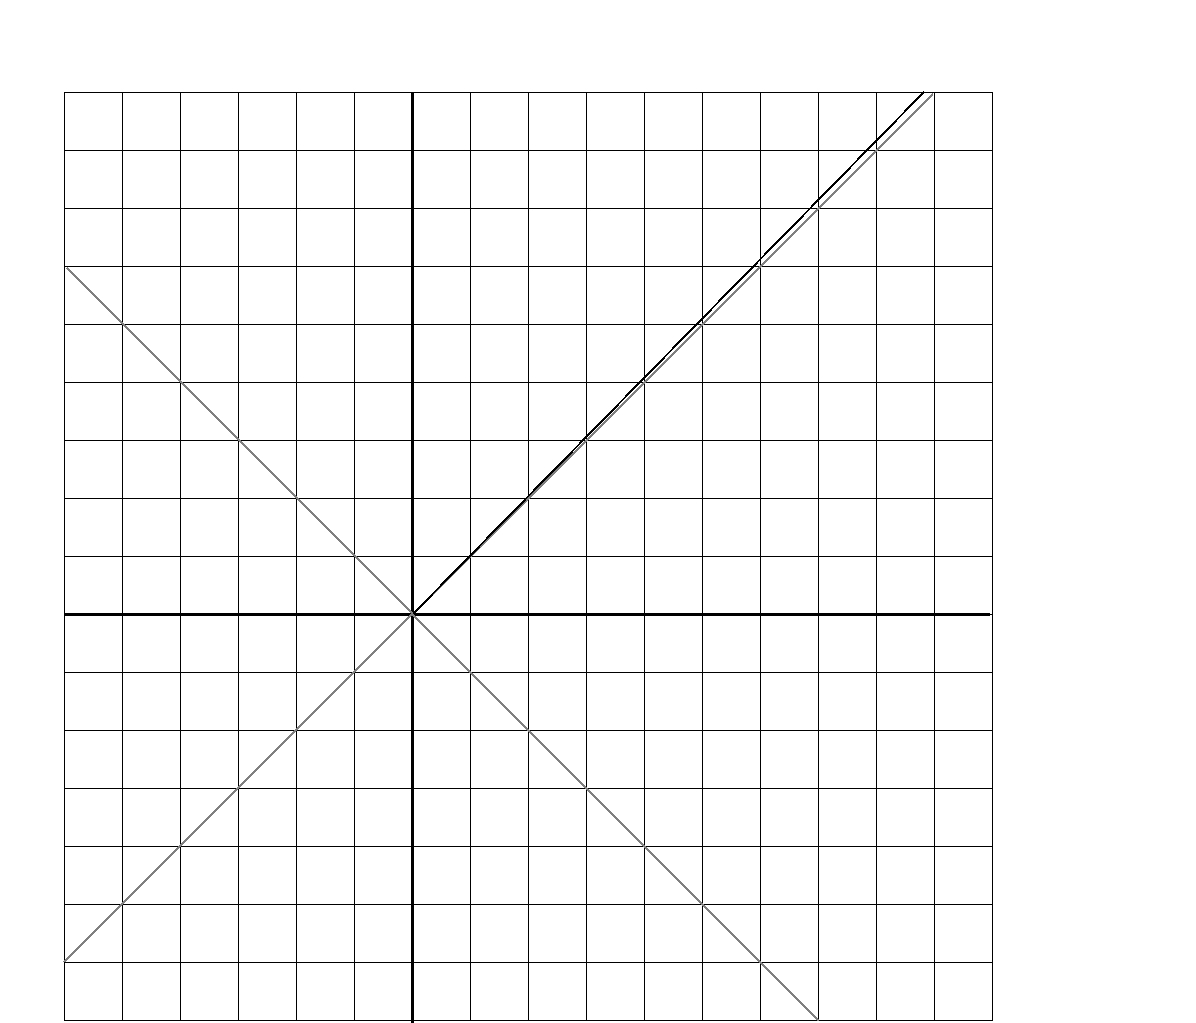
\includegraphics[width=0.68\textwidth]{Minkowski_Saccent.png}
%	\caption{Bijlagen bij vraag 3h).}
%	\label{fig:raketten}
%\end{figure}
%
%\begin{figure}[h]
%	\centering
%		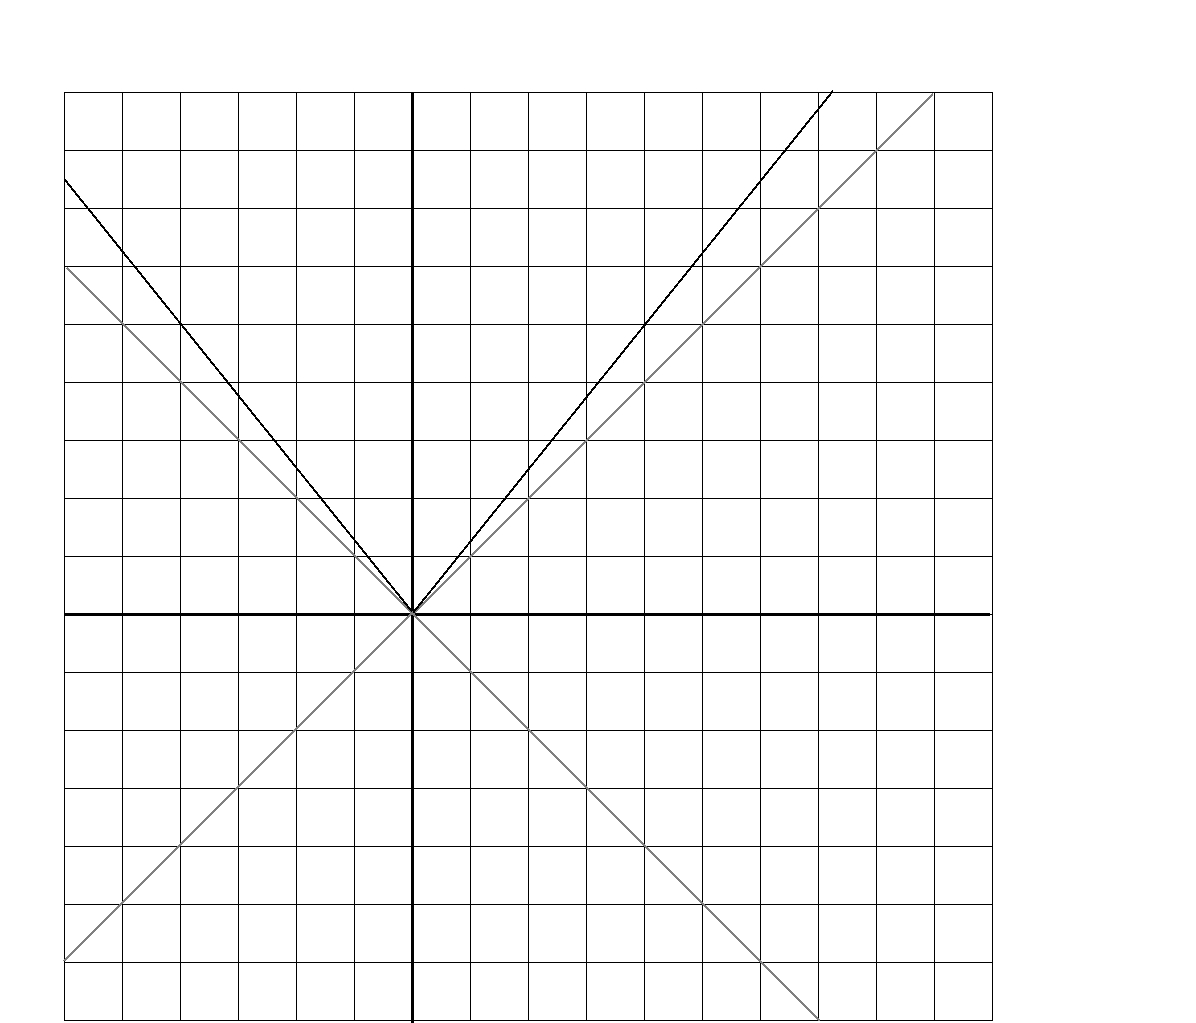
\includegraphics[width=0.68\textwidth]{Minkowski_S.png}
%	\caption{Bijlagen bij vraag 3h).}
%	\label{fig:raketten2}
%\end{figure}


%%%%%%%%%%%%
%\subsection{}
%In  het  Minkowski diagram in figuur \ref{} zijn de co\"{o}rdinaat-assen voor twee 
%inertiaalstelsels $S$ en 
%$S'$  getekend  die  een  onderlinge  snelheid langs de $x$-as hebben. 
%Voor de tijdseenheden kunnen 
%jaren worden gelezen, voor de lengte eenheden lichtjaren. 
%\begin{itemize}
%\item [a.]
%  Ga na dat die snelheid gelijk is aan $c/5$.
%\item [b.] 
%  Geef  met  een lijnstuk $OP$ geeft de reis aan van iemand ($B$) die twee 
%jaar met $S'$ mee beweegt. 
%  In $S$ blijft iemand anders ($A$) achter. 
%  Hoeveel tijd is er volgens A verlopen ($ct_{1}$) als de klok van B op c$t_{2}$=2 (jaar) staat? Loopt 
%  de tijd in $S_{2}$ volgens A te snel of te langzaam? 
%\end{itemize}
%  c)  Welk  tijdstip ($ct_{1}$) wijst de klok van A volgens B aan, als de klok van B op c$t_{2}$=2 staat? 
%  Loopt de tijd in $S_{1}$ volgens B te snel of te langzaam? 
%In  P  keert  B  om en beweegt met een even grote snelheid (-5c) terug naar A. Hij bereikt A in 
%punt Q. 
%  d) Teken de x3,ct3 assen door de oorsprong die voor het stelsel $S_{3}$ gelden waarin B zich op de 
%  terugreis bevindt. 
%  e)  Zodra  B  in  punt  P  aan  de  terugreis  begint  (en dus plotseling in stelsel $S_{3}$ zit), 
%  verspringt volgens hem de klok van A. Welke $ct_{1}$ ziet B dan? 
%  f) Hoeveel tijd duren de heen- en terugreis volgens B zelf? 
%  g) Hoeveel tijd is er volgens A voor de hele reis nodig geweest? 
%  In  de  vragen  b)  en c) was het zo dat A en B van elkaar vonden dat de klok van de ander te 
%  langzaam  ging.  Nu ze weer bij elkaar zijn, blijkt dat er voor B minder tijd is verlopen dan 
%  voor A (dit is de tweelingparadox). 
%  h) Waarom heeft B er geen recht op om te zeggen dat de tijd in A te langzaam liep? 
